\section{Introduction}

\subsection{Motivation}

\indent The exponential growth of client-server distributed applications has led to a need for them to be scalable systems able to service many users. Many applications currently rely on static configurations or topologies, which could limit their ability to change scale and adapt to changes in traffic. This inflexibility potential could cause increased latency and even service outages. This is because static topology configurations can perform well overall depending on the situation; however; for the internet, there is not a one size fits all solution, and a simple switch of topology to compensate for weaknesses of the previous could lead to a tremendous performance and robustness increase. For example, popular client-server distributed applications like Zoom struggled during the early COVID-19 pandemic because their current infrastructure limited their scalability, fault-tolerance, and efficiency during the surge of the increased nodes and geographical distribution of nodes. Ultimately, this problem that plagued the video calling platforms was fixed using edge computing and CDNs; however, they could have scaled by changing topology.

\indent This leads to the question: How does switching the nodes' topology affect the performance without negatively impacting the user's experience in a distributed client-server application? It is imperative to address this problem to ensure the continued growth of client-server distributed applications to maintain user satisfaction. 

\indent If this study can conclude that switching a topology could provide performance boosts for an application, it opens up the way for developing solutions to dynamically manage the topology's structure to leverage those performance boosts. Therefore, increasing the performance and scalability of future applications. In addition, the implications of this study could be the increased use of client-server technology in distributed applications, as businesses may be interested in its increased performance and reliability. It could also contribute to the understanding and previously unknown insights into client-server networks. Lastly, It could be of value to researchers working on related topics leading to even more innovation in the future.

\subsection{Methods of Changing Topologies}

\indent At the current moment, topology is reconfigurable through the use of an Optical Transport Network (OTN). Software-Defined Networking (SDN) and optical switches can change these fiber connections. SDNs are part of the network stack that decides the routing for packets for each router which, therefore, can change the topology of a network by simply changing the routes for packets. OTN is a protocol that allows optical networks a reliable and efficient way of transporting data across a network. Furthermore, optical switches can change the topology by directly switching one optical signal to another. Thus, this study will explore the switching of topologies under these methods.

\subsection{Outline}



\begin{figure}[tp]
\centering
\includegraphics[width=0.5 \textwidth]{figures/switches}
\caption{hye}
\end{figure}

\section{Related Work}
%\blindtext

And we need some citation here\cite{floyd1993random, stoica2001chord}

%\Blindtext

\section{System Design}

\indent To test if changing the topology affects the performance of a distributed system, we will test multiple topologies with different client-server setups and then change the topology and compare the performance metrics between them. To accomplish this goal, we will simulate a distributed system on top of an actual topology from The Internet Topology Zoo called AGIS. For the distributed system that is being simulated, we are using the benchmark TPC-H made by the Transaction Process Preformance Council (TPC).

\indent We use the AGIS topology for the simulation to reflect a real-world client-server system. Therefore, for transmitting data across the network, we only consider propagation delay calculated using the haversine distance between the coordinates of each edge of the graph.

\indent The TPC-H benchmark comes with a database generator with business-related queries and data modifications that simulate distributed systems involving data warehousing, business intelligence, decision support systems, and online analytical processing. Therefore, the reason for including TPC-H is to simulate these groups of distributed systems in a distributed environment closely related to those in the real world.

\indent The relevant metrics from TPC-H that will be used are power tests, throughput tests, and queries per hour. The power test measures how fast a single full stream of queries generated for TPC-H can be executed. The throughput test measure how fast multiple steams of queries can be executed. Lastly, the quries per hour convey how many queries can be satisfied over the course of an hour. These measurements are helpful in our study because we can compare the times and queries per hour with our original topology to another to conclude if there are any performance benefits.

\begin{figure}[tp]
\centering
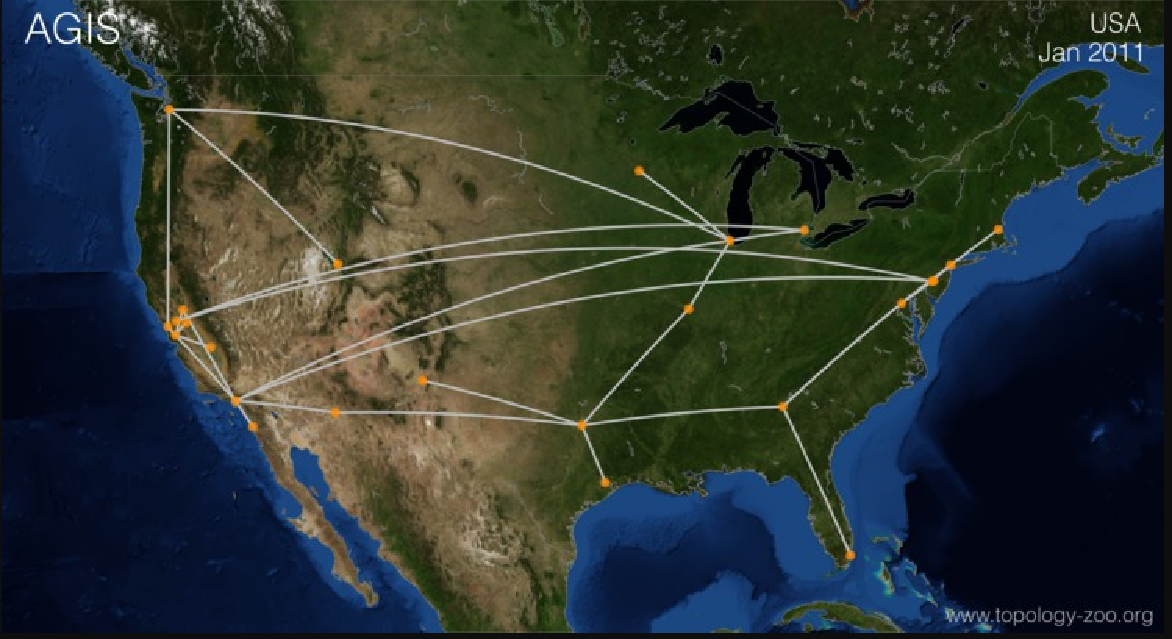
\includegraphics[width=0.5 \textwidth]{figures/AGIS_ORIG}
\caption{hye}
\end{figure}

\subsection{Simulations}

\subsection{One Server One Client Scenario}

\begin{figure}[tp]
\centering
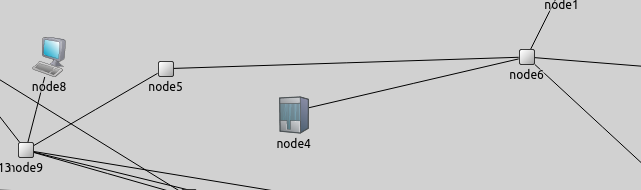
\includegraphics[width=0.5 \textwidth]{figures/SingleClientOrig}
\caption{hye}
\end{figure}

\begin{figure}[tp]
\centering
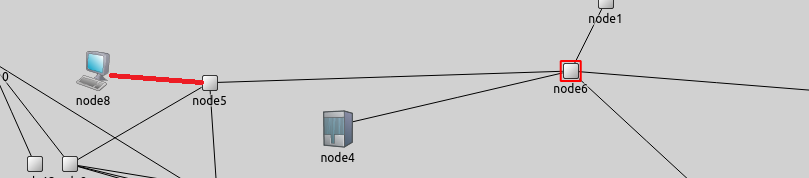
\includegraphics[width=0.5 \textwidth]{figures/SingleClientNew}
\caption{hye}
\end{figure}

\begin{table}[h!]
\centering
\begin{tabular}{|c|c|c|}
\hline
Server & Old Topology QPH@0.01 & New Topology QPH@0.01 \\ \hline
Server 0 & 247.2 & 249 \\ \hline
\end{tabular}
\caption{Queries per hour at scale factor 0.01 for Server 0 under old and new topologies}
\label{tab:my_label}
\end{table}


\begin{table}[h!]
\centering
\begin{tabular}{|c|c|c|}
\hline
Topology & Average Time (Seconds) \\ \hline
Old & 3.15 \\ \hline
New & 3.07 \\ \hline
\end{tabular}
\caption{Average time to service all clients under old and new topologies}
\label{tab:avg_time_all_clients}
\end{table}



\subsection{One Server Multi-Client Scenario}

\begin{figure}[tp]
\centering
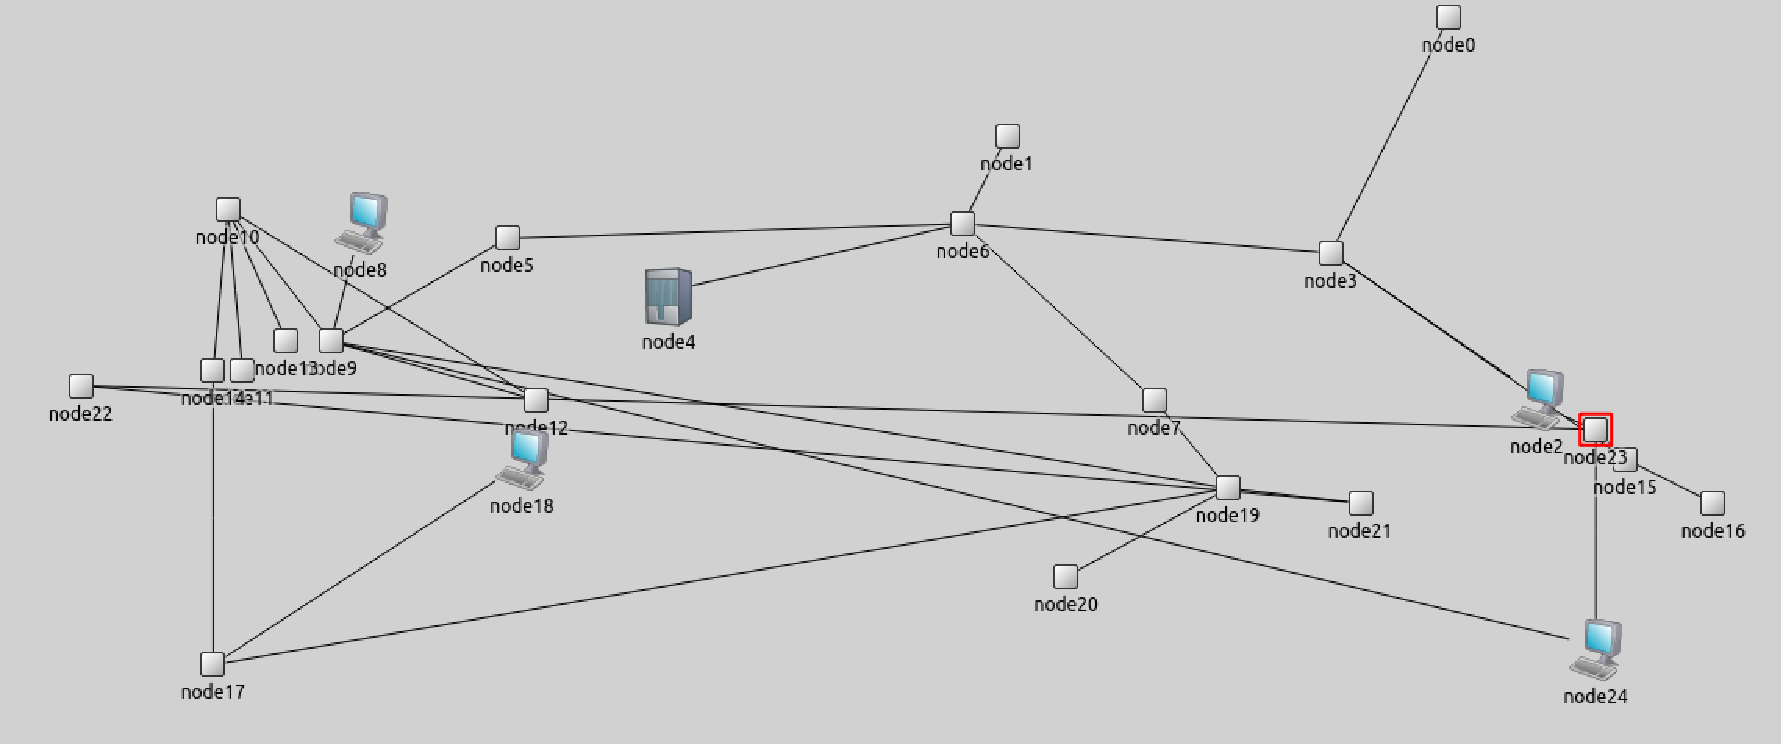
\includegraphics[width=0.5 \textwidth]{figures/MultClientOrig}
\caption{hye}
\end{figure}

\begin{figure}[tp]
\centering
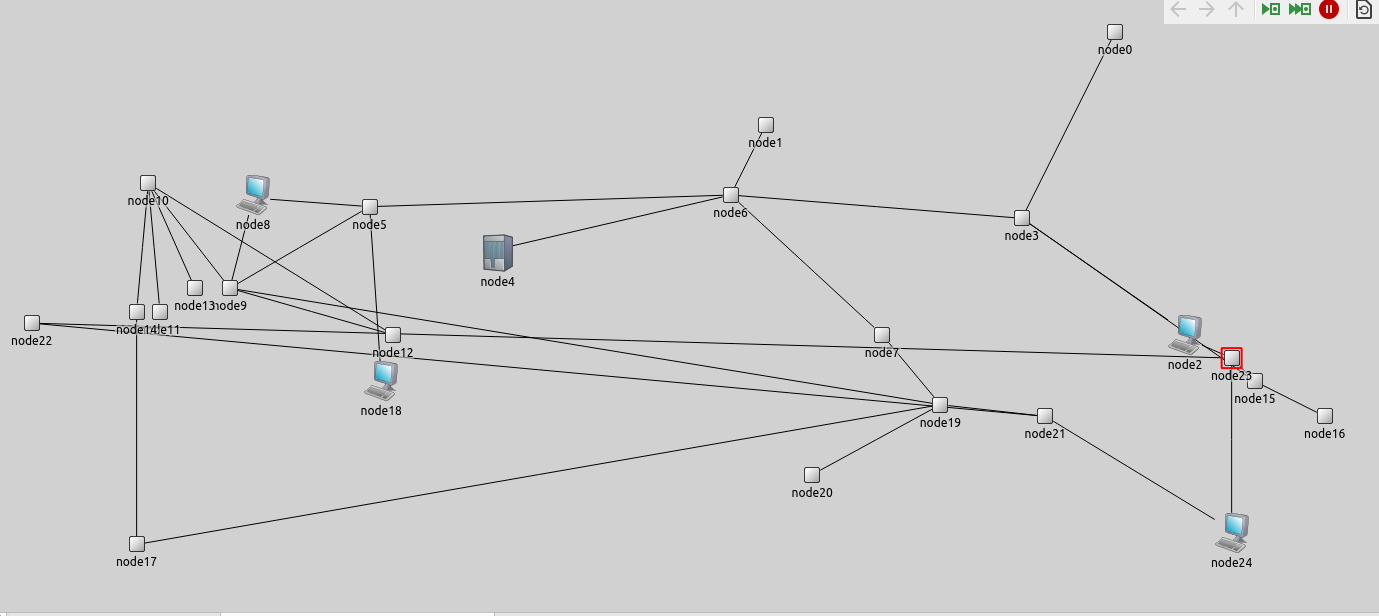
\includegraphics[width=0.5 \textwidth]{figures/MultClientNew}
\caption{hye}
\end{figure}

\begin{table}[h!]
\centering
\begin{tabular}{|c|c|c|}
\hline
Server & Old Topology QPH@0.01 & New Topology QPH@0.01 \\ \hline
Server 0 & 318.6 & 333 \\ \hline
\end{tabular}
\caption{Queries per hour at scale factor 0.01 for Server 0 under old and new topologies}
\label{tab:my_label}
\end{table}


\begin{table}[h!]
\centering
\begin{tabular}{|c|c|c|}
\hline
Server & Old Topology (s) & New Topology (s) \\ \hline
Server 0 & 3.15 & 3.07  \\ \hline
\end{tabular}
\caption{Average time to service all clients for Server 0 under old and new topologies}
\label{tab:average_time}
\end{table}

\begin{table}[h!]
\centering
\begin{tabular}{|c|c|c|}
\hline
Client Node & Old Topology (s) & New Topology (s) \\ \hline
Node 2 & 7.74 & 9.22  \\ \hline
Node 8 & 8.52 & 9.47 \\ \hline
Node 18 & 10.39 & 9.91 \\ \hline
Node 24 & 8.72 & 9.76 \\ \hline
\end{tabular}
\caption{Average time for each client node to complete its set of queries under old and new topologies}
\label{tab:avg_time_per_node}
\end{table}


For the first simulation, we consider a 4-client 1-server scenario; each is randomly assigned a geographic location, as shown in FIGURE 3. We first conducted 10 throughput tests, which yielded an average time of BLANK for each client for all of the client's queries to be satisfied by the server and returned to the client nodes. 

\subsection{Multi-Server Multi-Client Scenario}

\begin{figure}[tp]
\centering
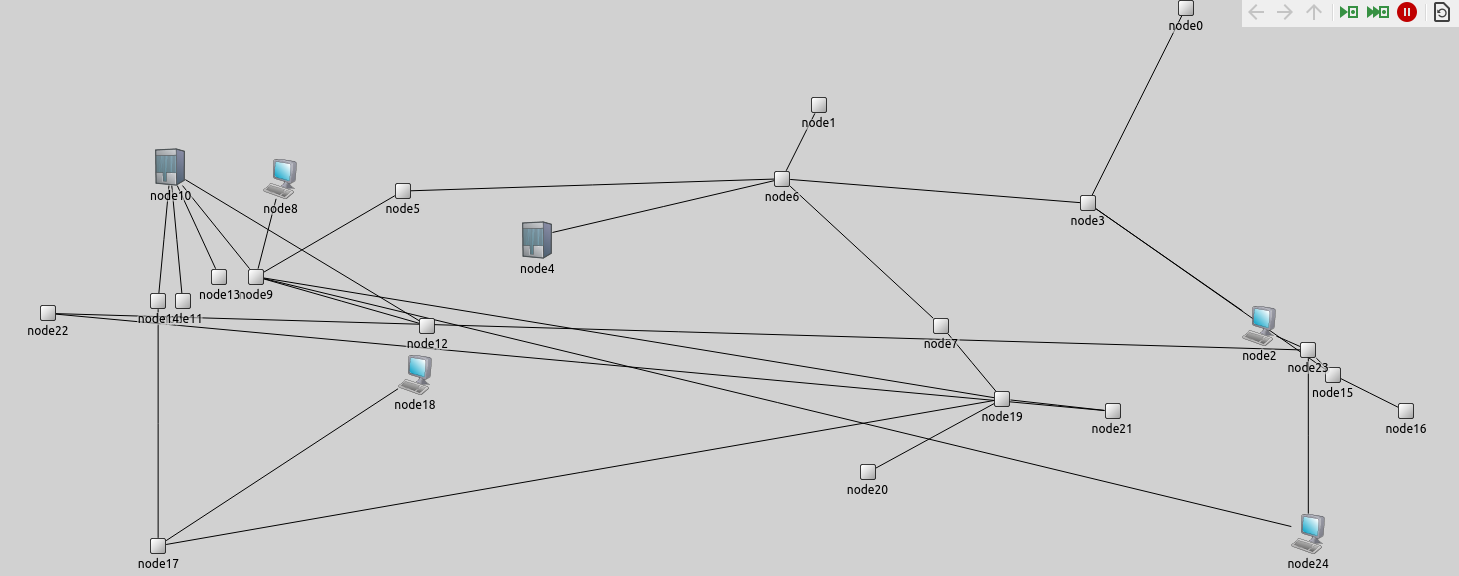
\includegraphics[width=0.5 \textwidth]{figures/MultServerOrig}
\caption{hye}
\end{figure}

\begin{figure}[tp]
\centering
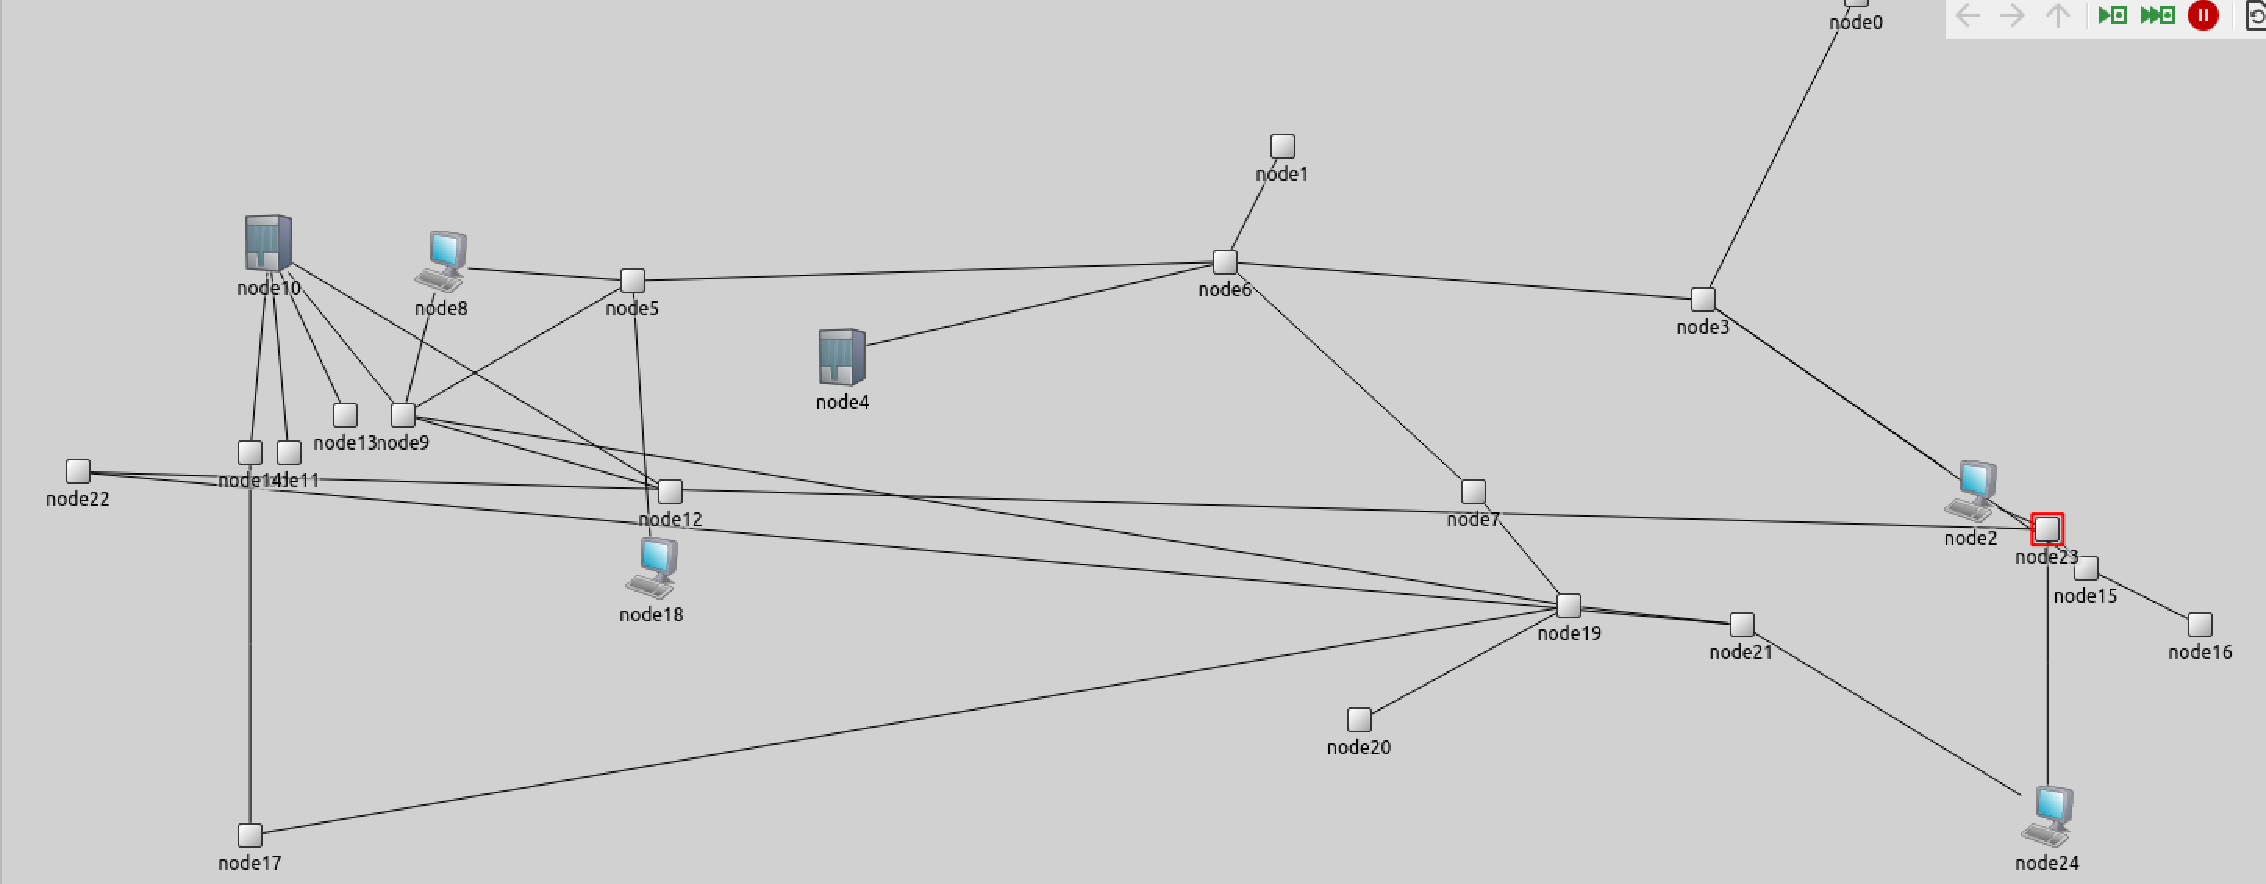
\includegraphics[width=0.5 \textwidth]{figures/MultServerNew}
\caption{hye}
\end{figure}

\begin{table}[h!]
\centering
\begin{tabular}{|c|c|c|}
\hline
Server & Old Topology QPH@0.01 & New Topology QPH@0.01 \\ \hline
Server 0 & 333.6 & 340.2  \\ \hline
Server 1 & 331.2 & 327 \\ \hline
\end{tabular}
\caption{Queries per hour at scale factor 0.01 for each server under old and new topologies}
\label{tab:my_label}
\end{table}

\begin{table}[h!]
\centering
\begin{tabular}{|c|c|c|}
\hline
Server & Old Topology (s) & New Topology (s) \\ \hline
Server 0 & 10.24 & 8.01  \\ \hline
Server 1 & 10.29 & 10.22 \\ \hline
\end{tabular}
\caption{Average time for each server to fulfill the client's queries under old and new topologies}
\label{tab:my_label}
\end{table}


\begin{table}[h!]
\centering
\begin{tabular}{|c|c|c|}
\hline
Client/Servers Nodes & Old Topology (s) & New Topology (s) \\ \hline
Client 2 Server 4 & 8.01  & 9.82  \\ \hline
Client 2 Server 10 & 10.22 & 10.29 \\ \hline
Client 8 Server 4 & 8.85  & 9.55  \\ \hline
Client 8 Server 10 & 4.98  & 4.67  \\ \hline
Client 18 Server 4 & 10.56 & 10.08 \\ \hline
Client 18 Server 10 & 7.61  & 7.73  \\ \hline
Client 24 Server 4 & 9.03  & 10.23 \\ \hline
Client 24 Server 10 & 10.1  & 10.12 \\ \hline
\end{tabular}
\caption{Average time for client node to complete its set of queries in old and new topology}
\label{tab:my_label}
\end{table}


\section{Discussion}
%\Blindtext

\section{Conclusion}
%\blindtext

